\chapter{Intrinsic Properties and Scattering Mechanisms}\label{chap:results}
Intro...

\section{Approach to Low-Resistance Contacts}\label{sec:contacts}
Developing low-resistance contacts is important two enable the study of intrinsic transport properties of devices, but also it is vital to applications of \acp{TMD}. Large contact resistance at room temperature is not ideal for applications. At the metal/semiconductor contact interface a barrier develops, the \acs{SB} \cite{Schottky_ZPhys1938}. The device in question must be able to supply the necessary current, and the voltage drop across the contacts should be small compared to the voltage drop across the device's active channel region. In most cases, the contacts should be ohmic, the current-voltage characteristic should be linear and not degrade the device's performance to any significant extent \cite{Rideout_Solid1975}. In the ideal, theoretical case (Schottky-Mott model)  the \acs{SBH} is given by 
\begin{equation}\label{eq:schottky_mott}
	\Phi_{\mathrm{B}p} = \frac{E_g}{e}- \left(\Phi_m - \chi_s\right),
\end{equation}
where $\Phi_{\mathrm{B}p}$ is the hole barrier height, $e$ is the charge of an electron, $E_g$ is the semiconductor bandgap energy, $\Phi_m$ is the metal workfunction, $\chi_s$ is the semiconductor electron affinity, note that these properties are intrinsic to the material before forming the junction \cite{Rhoderick_Book1988}. In reality the description is not this simple and is largely dependent on other factors, such as imperfections, Fermi level pinning, and Fermi level mismatch \cite{Cohen_Book2014}. For a metal/$p$-type semiconductor interface the magnitude of the \acs{SBH} is reflective of the mismatch in Fermi level of the metal and the \ac{VBM} of the semiconductor. Conversely, for the case of a metal/$n$-type interface it is the mismatch in the Fermi level of the metal and the \ac{CBM} of the semiconductor \cite{Tung_AppPhysRev2014}. Therefore, to address the issue of contact resistance one must find ways to effectively ``tune" the \acs{SB}.\\ \\

There have been several approaches employed in order to reduce the contact resistance. One method is to attempt to tune the \acs{SBH} by using different common metals to find a desirable work function. Eq.~\ref{eq:schottky_mott} implies that the \acs{SBH} is linearly dependent on the work function $\Phi_m$ of the metal. However, in reality, this is usually not the case because, one, finding metals with the proper work function that minimizes the \acs{SBH} while still maintaining high conductivity has proven to be difficult, and, two, the lowering that would potentially be achieved by the use of the proper work function would most likely be diminished due to Fermi level pinning \cite{Liu_ACSnano2012,Das_NanoLett2012,Liu_arxiv2016}. Fermi level pinning occurs when there are surface states that develop in the bandgap and pin the Fermi level position of the semiconductor \cite{Tung_AppPhysRev2014}. Another method is the use of graphene contacts \cite{HJ_Chuang_NanoLett2014,Das_NanoLett2014,Roy_ACSnano2014}. Barrier-free contacts have been achieved using this method in combination with \ch{MoS2} using a gate potential to tune band alignment \cite{Liu_NanoLett2015}. However, this method has not been shown to be extendable down to low enough contact resistances in some other \acp{TMD}, most notably \ch{WSe2}, but has been shown to be tunable down to $(<2\unita{k\Omega}\unita{\mu m}$) \cite{Chuang_2016,HJ_Chuang_NanoLett2014}. The method to that is enacted here to reduce the contact resistance is using degenerately doped contact regions. By degenerately doping the contact region one can thin the \acs{SB} width. However, this method is not without its challenges as well. Several doping techniques that can be used have limited spatial resolution \cite{Farmanbar_arxiv2016}. Depsite the challenges posed, this method has produced promising results that are transferrable to \acp{TMD} including \ch{WSe2}, \ch{MoS2}, and \ch{MoSe2} resulting in high-performance, low contact resistance devices. \\ \\

To determine the contact resistance of fabricated devices a method known as \ac{TLM} is used. In general, resistance is given by
\begin{equation}\label{eq:resistance_general}
	R = \frac{\rho}{A}l,
\end{equation}
where, in this case, it is assume that the resistivity $\rho$ and the area $A$ of the electrodes are constant throughout the device \cite{Schroder_Semiconductor2006}. The resistance $R$ is then proportional to the length of the channel $l$. By determining the resistance as a function of length one can deduce the contact resistance. The total contact resistance is given by
\begin{equation}\label{eq:contact_r}
	R = R_\mathrm{ch} + 2R_\mathrm{c},
\end{equation} 
where $R_\mathrm{c}$ and $R_\mathrm{ch}$ are the contact and channel resistances, respectively \cite{Schroder_Semiconductor2006}. A typical device for a \acs{TLM} measurement has drain and source electrodes with varying lengths between them. By find the resistance from the gradient of an $IV$ characteristic curve, one can apply the logic from eqs.~\ref{eq:resistance_general} and \ref{eq:contact_r} to find the contact resistance. The contact resistance is ultimately extracted from the $y$-intercept of a linear fit of resistance as a function of length for the device. In general, this method is done at several temperatures to further characterize the quality of the contacts as one would expect that at low temperatures, for low-resistance contacts, they would behave in similar fashion as they did at higher temperatures. To determine the affect that varying doping schemes has on contact resistance devices that were lightly doped (\lightlyfive) were measured using \acs{TLM} and compared to degenerately doped devices (\degenerate).

\subsection{Transmission Line Method: \lightlyfive}\label{subsec:TLM_lightly}
As stated in sec.~\ref{sec:contacts}, the \acs{TLM} measurement involves designing a device that has varying drain source channel lengths in order to determine the resistance as a function of length. Fig.~\subref*{fig:transmission_device_10232015_no1} shows an optical micrograph consisting of a lightly doped \ch{WSe2} (\lightlyfive) channel. Figs.~\subref*{fig:tlm_resistance1}-\subref*{fig:tlm_resistance3} show the total resistance as a function of length for both $V_{bg}=0\unita{V}$ and $V_{bg}=-60\unita{V}$ at room temperature. The contact resistance are then determine from the linear fit and the $y$-intercept. These figures show ohmic contacts with a minimum contact resistance of $R_\mathrm{c}=2.35\unita{k\Omega}\unita{\mu m}$ achieved with application of $V_{bg}=-60\unita{V}$. In addition, the contact resistances are lower for the higher values of $V_{bg}$. This is due, in part, to the fact that the higher $V_{bg}$ works to reduce the width of the \acs{SB} and allow for more transmission across the barrier that has developed between the metal/semiconductor interface. Moreover, when there is no $V_{bg}$ applied, the reported contact resistances are an order of magnitude higher. The fact that the channel material in use here is only lightly doped means that there is a larger mismatch between the Fermi level of the metal and the \acs{VBM} causing a larger \acs{SBH} than one would expect with a channel that was more heavily doped.
\begin{figure}[ht]
	\centering
	\subfloat[]{
		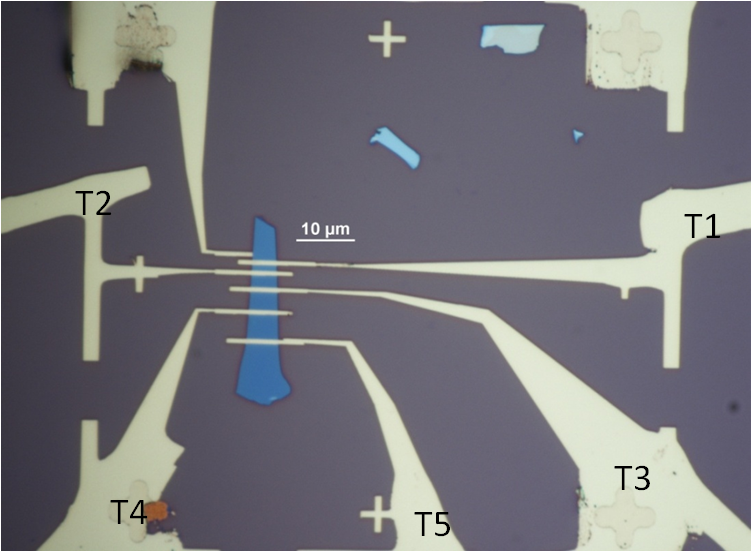
\includegraphics[height=4.25cm,width=5.0cm]{figs/results/transmission_line/transmission_device_pic_5-5_21_10232015_no1}
		\label{fig:transmission_device_10232015_no1}
	}
	\subfloat[]{
		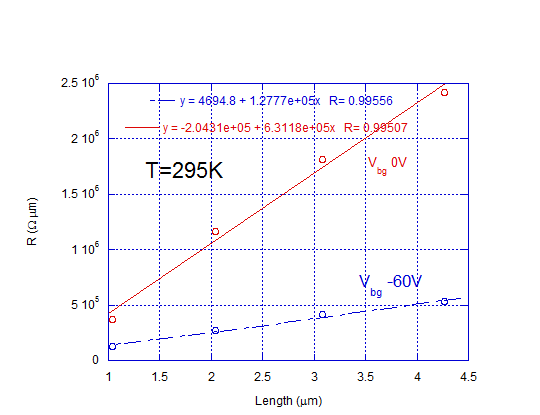
\includegraphics[height=4.25cm,width=5.0cm]{figs/results/transmission_line/transmission_resistance_plot_pic_5-5_21_10232015_no1}
		\label{fig:tlm_resistance1}
	}

	%\qquad
	\subfloat[]{
		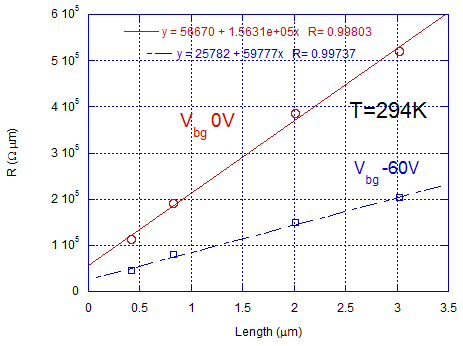
\includegraphics[height=4.25cm,width=5.0cm]{figs/results/transmission_line/transmission_resistance_plot_pic_56_21_10232015_no2}
		\label{fig:tlm_resistance2}
	}
	\subfloat[]{
		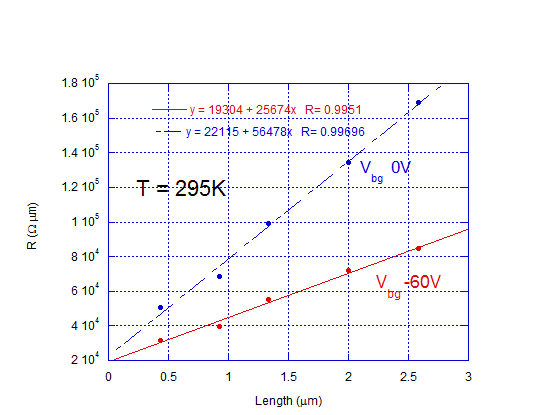
\includegraphics[height=4.25cm,width=5.0cm]{figs/results/transmission_line/transmission_resistance_plot_pic_-66_21_11182015_no2}
		\label{fig:tlm_resistance3}
	}
	\caption[TLM: contact resistances using \lightlyfive]{\protect\subref{fig:transmission_device_10232015_no1} Optical micrograph of a device structure for \acs{TLM} measurement consisting of lightly $p$-doped \ch{WSe2} (\lightlyfive) with \ch{Ti}/\ch{Au} metal contacts. \protect\subref{fig:tlm_resistance1}-\protect\subref{fig:tlm_resistance3} Normalized total resistance as a function of channel length measured at room temperature.}
	\label{fig:tlm_resistance_measurement_lightly}
\end{figure}

\subsection{Transmission Line Method: \degenerate}\label{subsec:TLM_degenerate}
The lightly doped \ch{WSe2} device showed reasonably low contact resistances at room temperature, but lower-resistance contacts are desired. Using \acs{TLM} degenerately doped \ch{WSe2} (\degenerate) devices were measured. Fig.~\subref*{fig:ben_tlm_resistance1} shows an optical micrograph of the device design which identical to that in sec.~\ref{subsec:TLM_lightly}. The contact resistances as a function of length are shown in figs.~\subref*{fig:ben_tlm_resistance2} and \subref*{fig:ben_tlm_resistance3} at room temperature and $5\unita{K}$, respectively. At both temperatures they exhibit linear ohmic behavior. Even more promising is that the values for contact resistance are essentially the same at high and low temperature, which indicates significant reduction of the \acs{SB}. The low temperature performance means that the contacts are of high quality as the contacts tend to degrade as temperature decreases mainly due to the lack of thermionic emmission of carriers \cite{Tung_AppPhysRev2014}. 
\begin{figure}[ht]
	\centering
	\subfloat[]{
		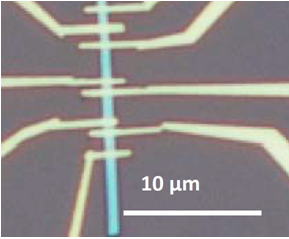
\includegraphics[height=4.25cm,width=5.0cm]{figs/results/transmission_line/ben_tlm_degenerately_doped_device_pic}
		\label{fig:ben_tlm_resistance1}
	}
	%\qquad
	\subfloat[]{
		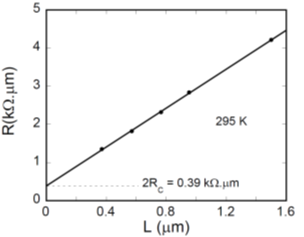
\includegraphics[height=4.25cm,width=5.0cm]{figs/results/transmission_line/ben_tlm_degenerately_doped_resistance_295K}
		\label{fig:ben_tlm_resistance2}
	}
	%\qquad
	\subfloat[]{
		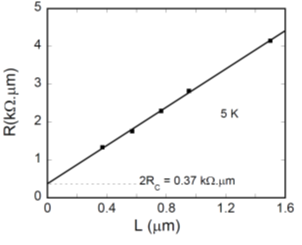
\includegraphics[height=4.25cm,width=5.0cm]{figs/results/transmission_line/ben_tlm_degenerately_doped_resistance_5K}
		\label{fig:ben_tlm_resistance3}
	}
	\caption[TLM: contact resistances using \degenerate]{\protect\subref{fig:ben_tlm_resistance1} Optical micrograph of a device structure for \acs{TLM} measurement consisting of degenerately $p$-doped \ch{WSe2} (\degenerate) with \ch{Ti}/\ch{Au} metal contacts. \protect\subref{fig:ben_tlm_resistance2} Normalized total resistance as a function of channel length measured at room temperature $T=295\unita{K}$ and \protect\subref{fig:ben_tlm_resistance3} low temperature $T=5\unita{K}$. Figures appeared in ref.~\cite{Chuang_2016}.}
	\label{fig:tlm_resistance_measurement_degenerate}
\end{figure}

\subsection{Discussion of Results for Light and Degenerately Doped Contacts}\label{subsec:contact_discussion}
The results for lightly (\lightlyfive) and degenerately (\degenerate) doped \ch{WSe2} contacts are summarized in table~\ref{table:contact_summary}. The degenerately doped contacts have resistances of at least an order of magnitude lower at room temperature due to the lowered \acs{SBH} from the higher doping scheme. The lightly doped contacts, though still relatively high, demonstrate the effect that applying a higher $V_{bg}$ can have on the \acs{SB}. An effective thinning of the barrier is observed for higher backgate voltage and thus this can also be used to further tune the \acs{SB} and lower contact resistances. The results from the lightly doped \ch{WSe2} channel are on the same order of magnitude as what has been previously shown using graphene/\ch{WSe2} contacts ($\sim 2\unita{k\Omega}\unita{\mu m}$) \cite{HJ_Chuang_NanoLett2014}. The results shown obtained for the degenerately doped \ch{WSe2} are significantly lower than graphene/\ch{WSe2} method and are in line with the best results that have been achieved for \acp{TMD} ($\sim 0.2-0.7\unita{k\Omega}\unita{\mu m}$ ) \cite{Yang_NanoLett2014,Kappera_NatureMat2014,Leong_ACSnano2014}. With these results in mind, this 2D/2D contact method using degenerately doped \ch{WSe2} (\degenerate) looks to be a viable and effective way to engineer low-resistance contacts which will be essential to explore the intrinsic channel properties of \acp{TMD}, the performance limits, and also when it comes to applications.
\begin{table}[ht]
	\centering
	\begin{threeparttable}
		\begin{tabular}{c c c}
			%\hline\hline
			\toprule
			Doping Content & Temperature ($\unita{K}$) & $R_\mathrm{c}(\unita{k\Omega}\unita{\mu m})$\tnote{$\ast$} \\ [0.5ex]
			%\hline
			\midrule
			$(0.05\%)$ \lightlyfive & 295 & $2.35$\tnote{$\dagger$}\\
			$(0.05\%)$ \lightlyfive & 294 & $12.9$\tnote{$\dagger$}\\
			$(0.05\%)$ \lightlyfive & 295 & $9.65$\tnote{$\dagger$}\\ 
			$(0.5\%)$ \degenerate & 295 & $0.195$\tnote{$\ddagger$}\\ 
			$(0.5\%)$ \degenerate & 5 & $0.185$\tnote{$\ddagger$}\\[1ex]
			%\hline
			\bottomrule
		\end{tabular}
		\begin{tablenotes}
			\item[$\ast$] The contact resistances $R_\mathrm{c}$ are reported as per electrode by taking the intercept and dividing by 2. In some other references this may not be the case.
			\item[$\dagger$] Resistance values from figs.~\subref*{fig:tlm_resistance1}, \subref*{fig:tlm_resistance2}, and \subref*{fig:tlm_resistance3}.
			\item[$\ddagger$] Resistance values from figs.~\subref*{fig:ben_tlm_resistance2} and \subref*{fig:ben_tlm_resistance3}.
		\end{tablenotes}
	\caption[Summary of contact resistances lightly $p$-doped and degenerately $p$-doped \ch{WSe2}]{Summary of contact resistances for lightly $p$-doped \ch{WSe2} (\lightlyfive) and degenerately $p$-doped \ch{WSe2} (\degenerate) found using linear fit data from figs.~\subref*{fig:tlm_resistance1}-\subref*{fig:tlm_resistance3} and \subref*{fig:ben_tlm_resistance2}-\subref*{fig:ben_tlm_resistance3}.}
	\label{table:contact_summary}
	\end{threeparttable}
\end{table}

\section{Field-Effect Mobility and Scattering Mechanisms}\label{sec:mufe_scatter}
There are several properties to electrically characterize and quantify the performance of a device. One such property is the two-probe and four-probe field-effect mobility $\mu_\mathrm{FE}$. The two-probe field-effect mobility is given by 
\begin{equation}\label{eq:mu_fe2}
	\mu_\mathrm{FE} = \frac{L}{w}\frac{1}{C}\frac{1}{V_{ds}}\frac{d I_{ds}}{V_{bg}},
\end{equation}
where $L$ is the length of the channel (the distance between the source and drain), $w$ is the width of the channel, $I_{ds}$ is the drain current, $V_{bg}$ is the backgate voltage, $V_{ds}$ is the drain voltage, and $C$ is the geometric capacitance \cite{Stassen_AppPhysLett2004}. To measure the field-effect mobility there are two main approaches used, either the two-probe method or the four-probe method. The two-probe method is shown in fig.~\subref*{fig:two_probe}. In this configuration measurement takes place between the drain and source only. The main drawback of this measurement is that it is subject to resistance that can make data difficult to interpret because of this \cite{Schroder_Semiconductor2006}. Alternatively, there is the four-point probe configuration which is shown in fig.~\subref*{fig:four_probe} \cite{Valdes_IRE1954}. The main advantage of this configuration is that the voltage drop is measured across $V_3$ and $V_2$ and therefore allows the resistance to be subtracted. The field-effect mobility is important to characterizing a device because, it can reveal information about scattering mechanisms present and how they affect the mobility. Also, depending on the device's channel and whether it is doped or not, the mobility shows how the doping can be tuned to perform in a desired manner for device applications, especially at room temperature. To begin to study these issues devices with varying doping schemes and fabrication methods were measured to address where improvements can be made and where unknowns still exist.
\begin{figure}[ht]
	\centering
	\subfloat[]{
		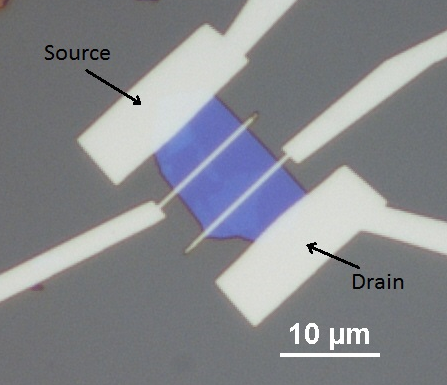
\includegraphics[height=4cm,width=4.75cm]{figs/-44_54_100x_after_liftoff_two_point_probe_measurement}
		\label{fig:two_probe}
	}
	\qquad
	\subfloat[]{
		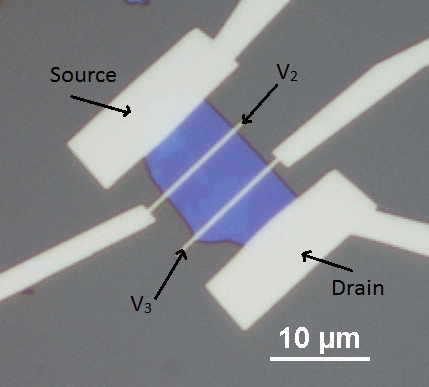
\includegraphics[height=4cm,width=4.75cm]{figs/-44_54_100x_after_liftoff_four_point_measurement}
		\label{fig:four_probe}
	}
	\caption[Field-effect mobility measurement configuration]{Examples of \protect\subref{fig:two_probe} two-point probe measurement configuration for field-effect mobility measurements and \protect\subref{fig:four_probe} four-point probe configuration.}
\end{figure}

\subsection{Applying Low-Resistance Contacts: Doped Channel}\label{subsec:mufe_doped_channel}
\begin{figure}[ht]
	\centering
	\subfloat[]{
		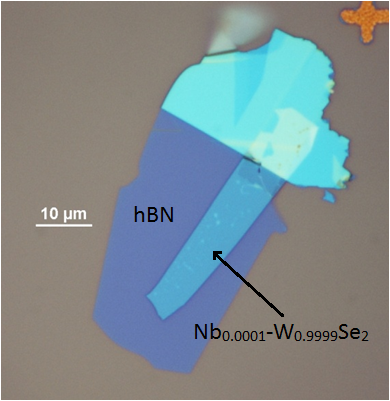
\includegraphics[height=3.75cm,width=3cm]{figs/results/hall_bar_doped_channel_doped_contacts/pWSe2_on_hBN_substrate_5-5_21_no1_annotated}
		\label{fig:pWSe2_doped_contacts_and_channel_step1}
	}
	\qquad
	\subfloat[]{
		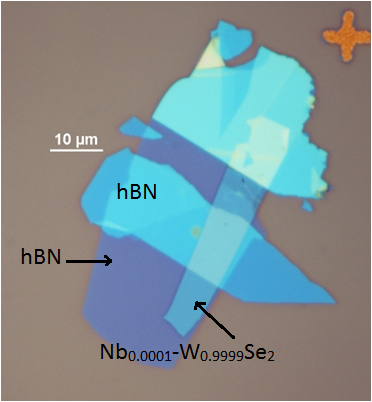
\includegraphics[height=3.75cm,width=3cm]{figs/results/hall_bar_doped_channel_doped_contacts/pWSe2_on_hBN_substrate_with_top_hBN_5-5_21_no1_annotated}
		\label{fig:pWSe2_doped_contacts_and_channel_step2}
	}
	\qquad
	\subfloat[]{
		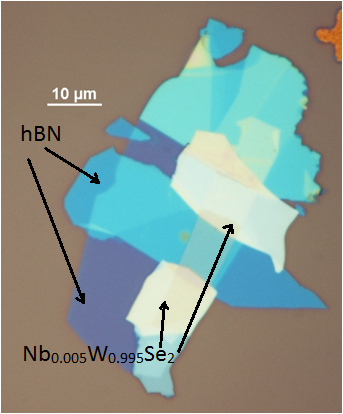
\includegraphics[height=3.75cm,width=3cm]{figs/results/hall_bar_doped_channel_doped_contacts/pWSe2_on_hBN_substrate_with_top_hBN_doped_contact_transfer_5-5_21_no1_annotated}
		\label{fig:pWSe2_doped_contacts_and_channel_step3}
	}
	\qquad
	\subfloat[]{
		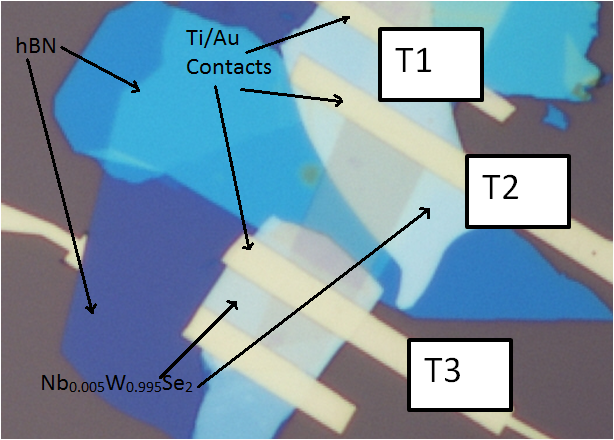
\includegraphics[height=3cm,width=3.75cm]{figs/results/hall_bar_doped_channel_doped_contacts/pWSe2_device_with_electrodes_5-5_21_no1_annotated}
		\label{fig:pWSe2_doped_contacts_and_channel_final_device}
	}
	\caption[Fabrication steps of \lightlyone channel with \degenerate\, contacts]{\protect\subref{fig:pWSe2_doped_contacts_and_channel_step1} \lightlyone transferred to \hbn substate,  \protect\subref{fig:pWSe2_doped_contacts_and_channel_step2} top \hbn transferred onto channel, \protect\subref{fig:pWSe2_doped_contacts_and_channel_step3} degenerately doped (\degenerate) contacts transferred onto device, and \protect\subref{fig:pWSe2_doped_contacts_and_channel_final_device} device after fabrication steps with \ch{Ti}/\ch{Au} metal electrodes consisting of a $5.6\unita{nm}$ thick channel.}
	\label{fig:hBN_field_effect_device_fab}
\end{figure}

\begin{figure}[ht]
	\centering 
	\subfloat[]{
		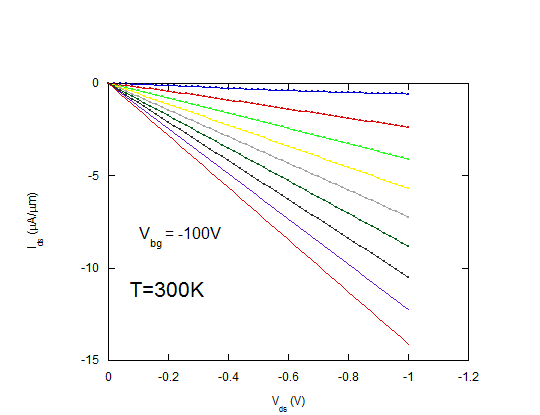
\includegraphics[height=4.55cm,width=5.3cm]{figs/results/hall_bar_doped_channel_doped_contacts/Vds-Id_Vds_1V_-1V-Vbg_-20V_-100V_T2-T3_300K-04_plot_before_anneal_5-5_21_no1}
		\label{fig:5-5_21_no1_pre_anneal_iv_300k}
	}
	\subfloat[]{
		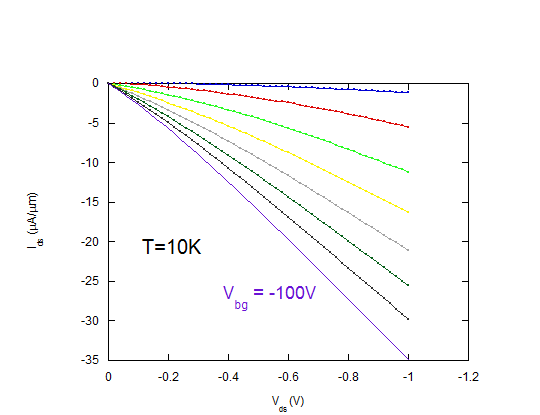
\includegraphics[height=4.55cm,width=5.3cm]{figs/results/hall_bar_doped_channel_doped_contacts/Vds-Id_Vds_1V_-1V-Vbg_-30V_-100V_T2-T3_10K-03_plot_before_anneal_5-5_21_no1}
		\label{fig:5-5_21_no1_pre_anneal_iv_10k}
	}
	\subfloat[]{
		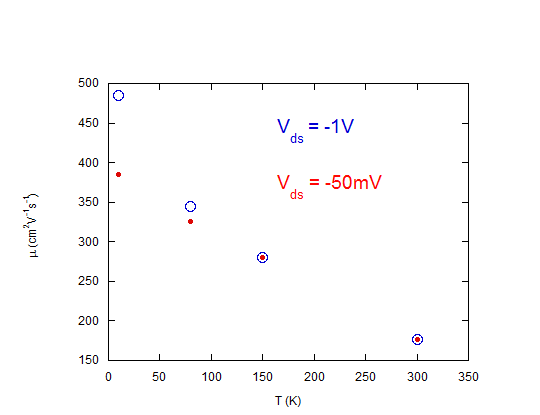
\includegraphics[height=4.55cm,width=5.3cm]{figs/results/hall_bar_doped_channel_doped_contacts/Two_Probe_FE_Mobility_Vs_T_Vds_-1V_-50mV_plot_pre_anneal_5-5_21_no1}
		\label{fig:5-5_21_no1_pre_anneal_mu_fe_vs_temp}
	}
	\caption[Characteristics of \ch{WSe2} \acs{FET} with lightly $p$-doped channel and 2D/2D contacts: I]{\protect\subref{fig:5-5_21_no1_pre_anneal_iv_300k} $IV$ chacteristics of device at $T=300\unita{K}$ and \protect\subref{fig:5-5_21_no1_pre_anneal_iv_10k} at $T=10\unita{K}$. \protect\subref{fig:5-5_21_no1_pre_anneal_mu_fe_vs_temp} Two-terminal field-effect mobility as a function of temperature for $V_{ds}=-50\unita{mV}$ and $-1\unita{V}$. \emph{Note: figures correspond to device shown in fig.~\subref*{fig:pWSe2_doped_contacts_and_channel_final_device}. Measurements shown were made before the device was annealed}.}
	\label{fig:pre_anneal_mu_fe_measurements}
\end{figure}

\begin{figure}[ht]
	\centering
	\subfloat[]{
		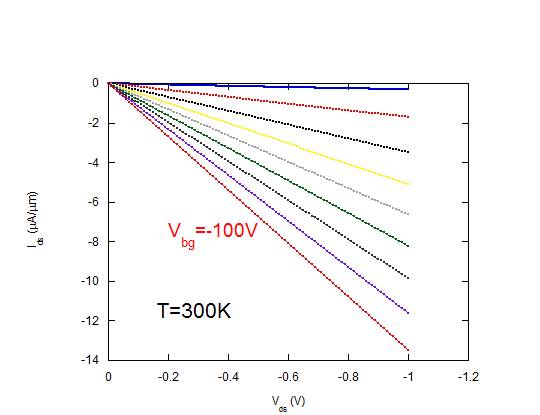
\includegraphics[height=4.55cm,width=5.3cm]{figs/results/hall_bar_doped_channel_doped_contacts/Vds-Id_Vds_1V_-1V-Vbg_-20V_-100V_T2-T3_300K-13_plot_after_anneal_5-5_21_no1}
		\label{fig:5-5_21_no1_post_anneal_iv_300k}
	}
	\subfloat[]{
		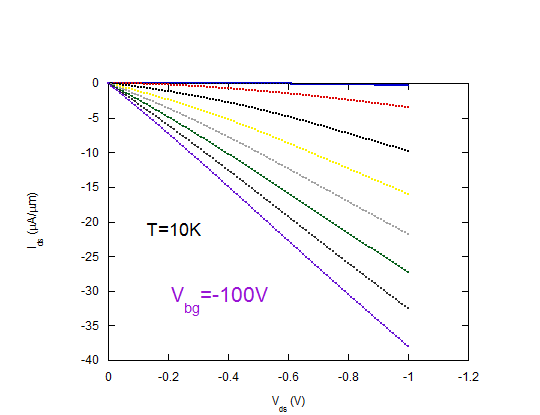
\includegraphics[height=4.55cm,width=5.3cm]{figs/results/hall_bar_doped_channel_doped_contacts/Vds-Id_Vds_1V_-1V-Vbg_-30V_-100V_T2-T3_10K-03_plot_after_anneal_5-5_21_no1}
		\label{fig:5-5_21_no1_post_anneal_iv_10k}
	}
	\subfloat[]{
		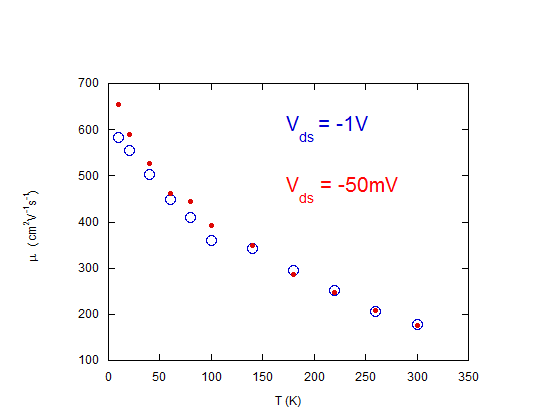
\includegraphics[height=4.55cm,width=5.3cm]{figs/results/hall_bar_doped_channel_doped_contacts/Two_Probe_FE_Mobility_Vs_T_Vds_-1V_-50mV_plot_post_anneal_5-5_21_no1}
		\label{fig:5-5_21_no1_post_anneal_mu_fe_vs_temp}
	}
	\caption[Characteristics of \ch{WSe2} \acs{FET} with lightly $p$-doped channel and 2D/2D contacts: II]{\protect\subref{fig:5-5_21_no1_post_anneal_iv_300k} $IV$ chacteristics of device at $T=300\unita{K}$ and \protect\subref{fig:5-5_21_no1_post_anneal_iv_10k} at $T=10\unita{K}$. \protect\subref{fig:5-5_21_no1_post_anneal_mu_fe_vs_temp} Two-terminal field-effect mobility as a function of temperature for $V_{ds}=-50\unita{mV}$ and $-1\unita{V}$. \emph{Note: figures correspond to device shown in fig.~\subref*{fig:pWSe2_doped_contacts_and_channel_final_device}. Measurements shown weree made after the device was annealed for 30 minutes at $250^\degree\unita{C}$}.}
	\label{fig:post_anneal_mu_fe_measurements}
\end{figure}

\subsection{Applying Low-Resistance Contacts: Undoped Channel}\label{subsec:mufe_undoped_channel}
\begin{figure}[ht]
	\centering
	\subfloat[]{
		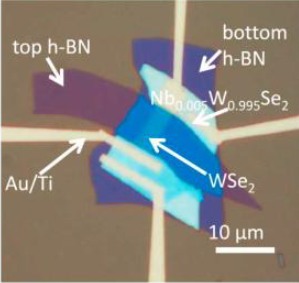
\includegraphics[height=4.5cm,width=5cm]{figs/results/ben/undoped_wse2_degen_doped_contacts}
		\label{fig:undoped_wse2_pic}
	}
	\subfloat[]{
		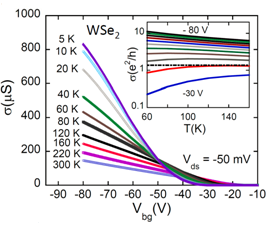
\includegraphics[height=4.5cm,width=5cm]{figs/results/ben/conductivity_2d2d_contacts_vs_Vbg_wse2}
		\label{fig:undoped_wse2_conduct}
	}
	\subfloat[]{
		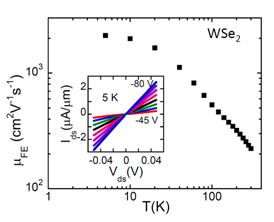
\includegraphics[height=4.5cm,width=5cm]{figs/results/ben/mu_fe_2d2d_contacts_vs_T_wse2}
		\label{fig:undoped_wse2_mu_fe}
	}
	\caption[Characteristics and channel properties of \ch{WSe2} \acs{FET} with 2D/2D contacts]{\protect\subref{fig:undoped_wse2_pic} Optical micrograph of \ch{WSe2} \acs{FET} with degenerately $p$-doped \ch{WSe2} (\degenerate) contacts with channel region on \hbn substrate and covered with a top \hbn piece. \protect\subref{fig:undoped_wse2_conduct} Temperature dependent two-terminal conductivity as a function of $V_{bg}$ at $V_{ds}=-50\unita{mV}$ for device shown in \protect\subref{fig:undoped_wse2_pic}. \protect\subref{fig:undoped_wse2_mu_fe} Two-terminal field-effect mobility. Figures appeared in ref.~\cite{Chuang_2016}.}
	\label{fig:mu_fe_data_degenerate}
\end{figure}

\section{Hall Effect and Applying Low-Resistance Contacts}\label{sec:hall_effect_intro}
\begin{figure}[ht]
	\centering
	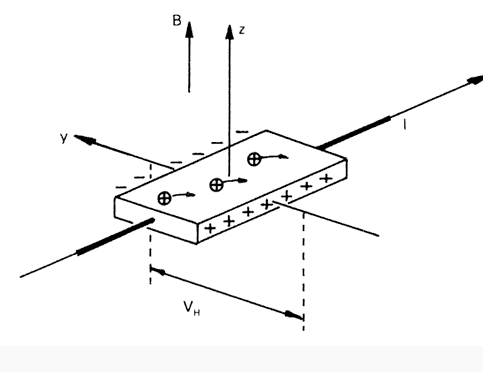
\includegraphics[height=6cm,width=8cm]{figs/results/hall_diagram}
	\caption[Hall effect measurement diagram]{Geometry of Hall effect measurement. Current flows in the positive $x$-direction and magnetic field is applied in the positive $z$ direction generating a Hall voltage \cite{HallEffectNIST}. Diagram originally appeared in ref.~\cite{HallDiagram}.}
	\label{fig:hall_diagram}
\end{figure}

\subsection{Hall Effect: \lightlyfive}\label{subsec:hall_lightly}
\begin{figure}[ht]
	\centering
	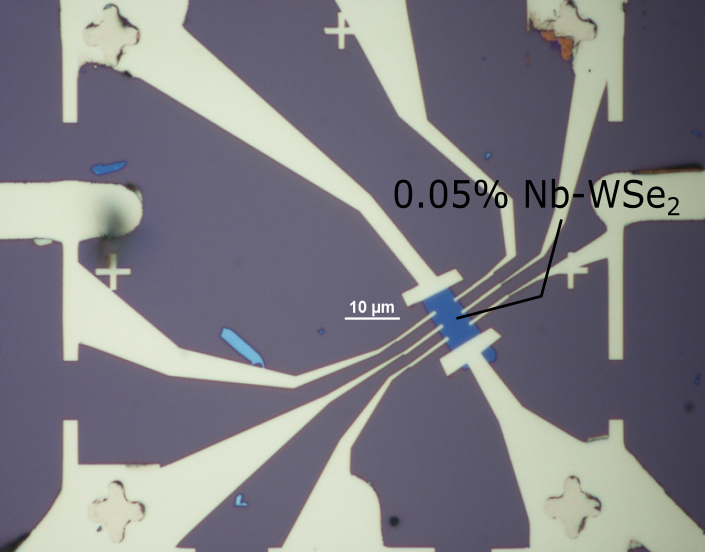
\includegraphics[height=4.5cm,width=6.0cm]{figs/results/hall_bar_doped_channel/hall_bar_device_pic_11192015_no2_doping_scheme}
	\caption[Hall bar device optical micrograph using \lightlyfive]{Optical micrograph of device structure consisting of lightly $p$-doped \ch{WSe2} (\lightlyfive) with device thickness $7.7\unita{nm}$ and \ch{Ti}/\ch{Au} metal contacts.}
	\label{fig:hall_bar_device1}
\end{figure}

\begin{figure}[ht]
	\centering
	\subfloat[]{
		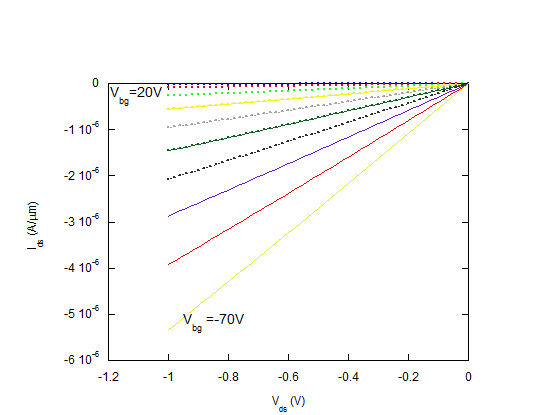
\includegraphics[height=4.25cm,width=5.0cm]{figs/results/hall_bar_doped_channel/Vds-Id_1V_-1V-Vbg_20V_-70V_T1-D_T5_S_300K_plot_modified_11192015_no2}
		\label{fig:11192015_ohmic_contacts}
	}
	%\qquad
	\subfloat[]{
		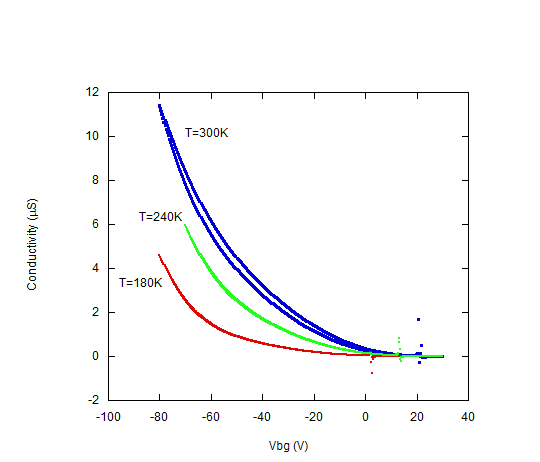
\includegraphics[height=4.25cm,width=5.0cm]{figs/results/hall_bar_doped_channel/hall_bar_device_pic_11192015_no1_conduct_vs_Vbg_all_temps}
		\label{fig:11192015_conduct_vs_temp}
	}
	\subfloat[]{
		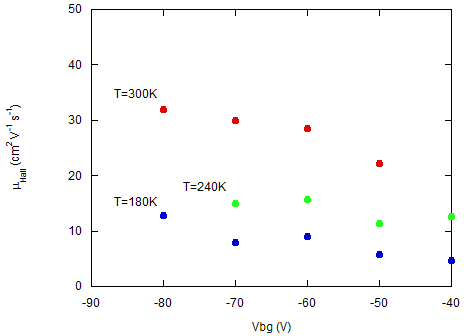
\includegraphics[height=4.25cm,width=5.0cm]{figs/results/hall_bar_doped_channel/hall_bar_device_pic_11192015_no1_mu_hall_vs_Vbg_all_temps}
		\label{fig:11192015_mu_hall_vs_temp}
	}

	%\qquad
	\subfloat[]{
		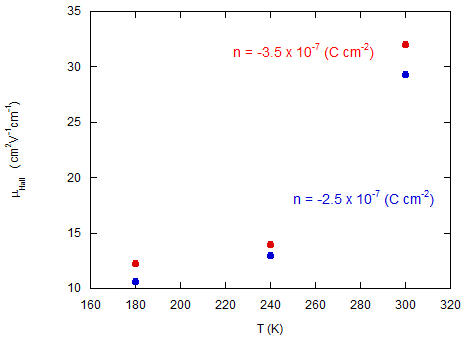
\includegraphics[height=4.25cm,width=5.0cm]{figs/results/hall_bar_doped_channel/HallMobility_Vs_T_for_fixed_carrier_consentrations_plot_modified_11192015_no2}
		\label{fig:11192015_mu_hall_vs_temp_various_n}
	}
	\qquad
	\subfloat[]{
		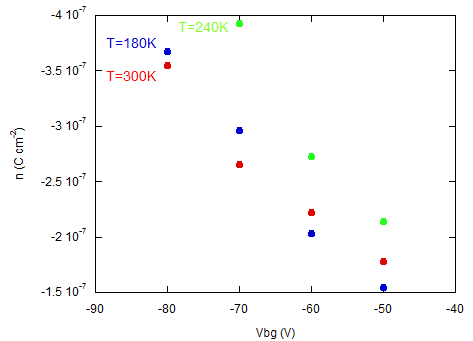
\includegraphics[height=4.25cm,width=5.0cm]{figs/results/hall_bar_doped_channel/Charge_density_Vs_Vbg_different_Temp_plot_modified_11192015_no1}
		\label{fig:11192015_n_vs_Vbg}
	}
	\caption[Output characteristics and channel properties of lightly $p$-doped \ch{WSe2} with 2D/2D contacts]{\protect\subref{fig:11192015_ohmic_contacts} $IV$ characteristic curve at $T=300\unita{K}$ as a function of $V_{ds}$ for $V_{bg}$ ranging from $-70\unita{V}$ to $20\unita{V}$. \protect\subref{fig:11192015_conduct_vs_temp} Temperature-dependence of conductivity and \protect\subref{fig:11192015_mu_hall_vs_temp} Hall mobility as a function of $V_{bg}$. \protect\subref{fig:11192015_mu_hall_vs_temp_various_n} Charge carrier denisty dependence of Hall mobility as a function of temperature and \protect\subref{fig:11192015_n_vs_Vbg} temperature dependence of charge carrier density as a function of $V_{bg}$. \emph{Note: the data here corresponds to device shown in fig.~\ref{fig:hall_bar_device1}}.}
	\label{fig:hall_measurement_data_lightly}
\end{figure}

\subsection{Hall Effect: Extended to Contact Method}\label{subsec:hall_degenerate}

\begin{figure}[ht]
	\centering
	\subfloat[]{
		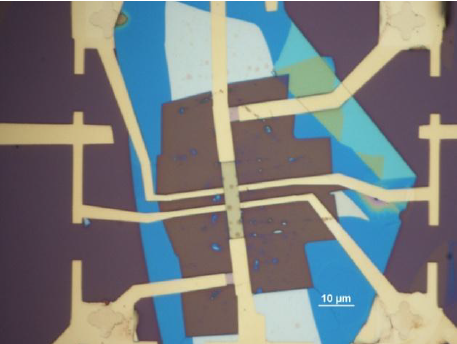
\includegraphics[height=4.75cm,width=5.5cm]{figs/results/ben/pWSe2_hall}
		\label{fig:pWSe2_hall}
	}
	\qquad
	\subfloat[]{
		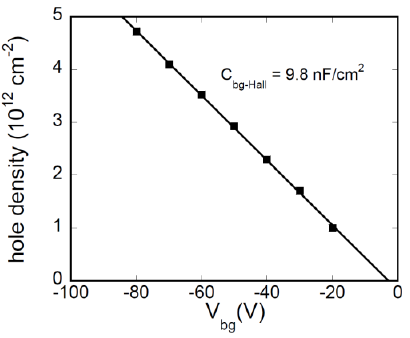
\includegraphics[height=4.75cm,width=5.5cm]{figs/results/ben/pWSe2_cap}
		\label{fig:pWSe2_cap}
	}
	\caption[Hall effect measurement with 2D/2D contacts to determine capacitance]{\protect\subref{fig:pWSe2_hall} Optical microgrpah of \ch{WSe2} Hall bar device encapsulated in \hbn with degenerate 2D/2D contacts. \protect\subref{fig:pWSe2_cap} Hole density as a function of $V_{bg}$ at $T=300\unita{K}$ extracted from Hall effect measurement. Figures appeared in ref.~\cite{Chuang_2016}.}
	\label{fig:pWSe2_hall_ben}
\end{figure}